\chapter{Agronegócio}
\par A agricultura é importante para o Brasil, é um setor que cresce de forma exponencial e alavanca a economia de inúmeros estados da federação. O agronegócio representou 21,4\% do \acrshort{pib} nacional em 2019, demonstrando o quão providencial é para o país. Já para o Tocantins, sua participação está abaixo da média nacional, com menos de 15\% do \acrshort{pib} estadual. Nesta sessão do Boletim apresenta-se os seguintes dados da agricultura; Área de produção, colhida, produção de cereais e oleaginosas e o seu rendimento médio. Em seguida, analise-se os dados de abates de animais, produção de ovos de galinha e leite.

% \section{Produção}
\par O estado do Tocantins utilizou 1.520.698 hectares do seu território para a produção agrícola no primeiro semestre de 2020. Dentre os 5 principais produtos plantados no estado, conforme a Figura \ref{fig:lavouras}, destaca-se a cana-de-açúcar e a soja com as maiores proporções, responsáveis por 38.2\% e 36.2\% do total produzido. O milho ocupa a terceira posição entre os produtos mais cultivados no estado neste período, com 14.5\%. A produção de arroz e mandioca também ganha destaque ao representar um montante de 8.2\% e 3\%, respectivamente, fechando assim o ranking dos cinco produtos com os melhores desempenhos na agricultura tocantinense.

\begin{figure}[!h]
	\begin{subfigure}{\linewidth}
		\caption{Produção das principais lavouras}
		\subcap{Em milhões de toneladas. Estimativa anual de setembro}
		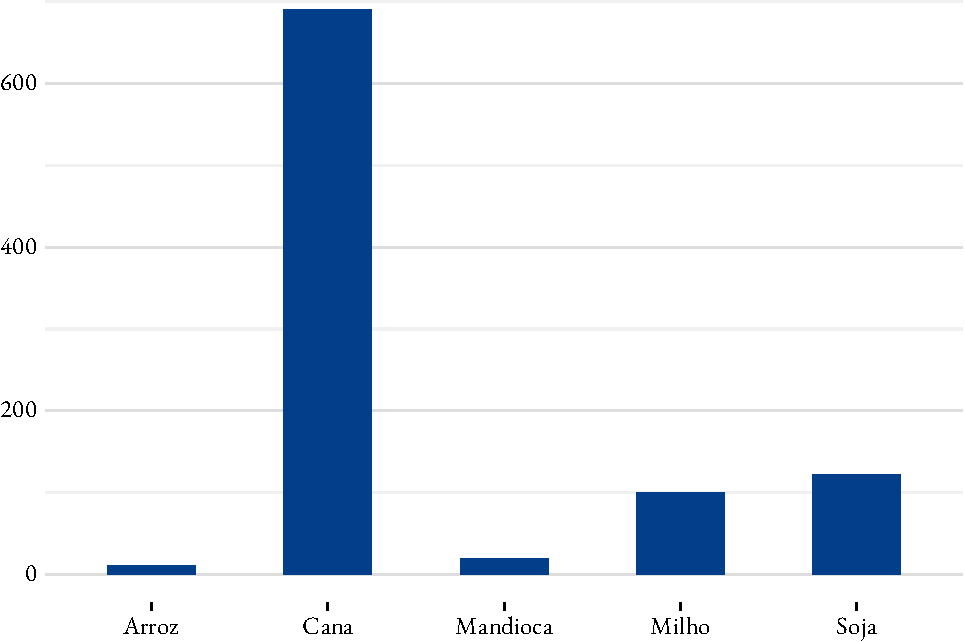
\includegraphics{fig/producao-1.pdf}
		\source{\acrshort{sidra}/\acrshort{ibge}}
		\label{fig:lavouras}
	\end{subfigure}
	\begin{subfigure}{\linewidth}
		\caption{Rendimento médio das lavouras}
		\subcap{Mil quilogramas por hectare. Estimativa anual de setembro}
		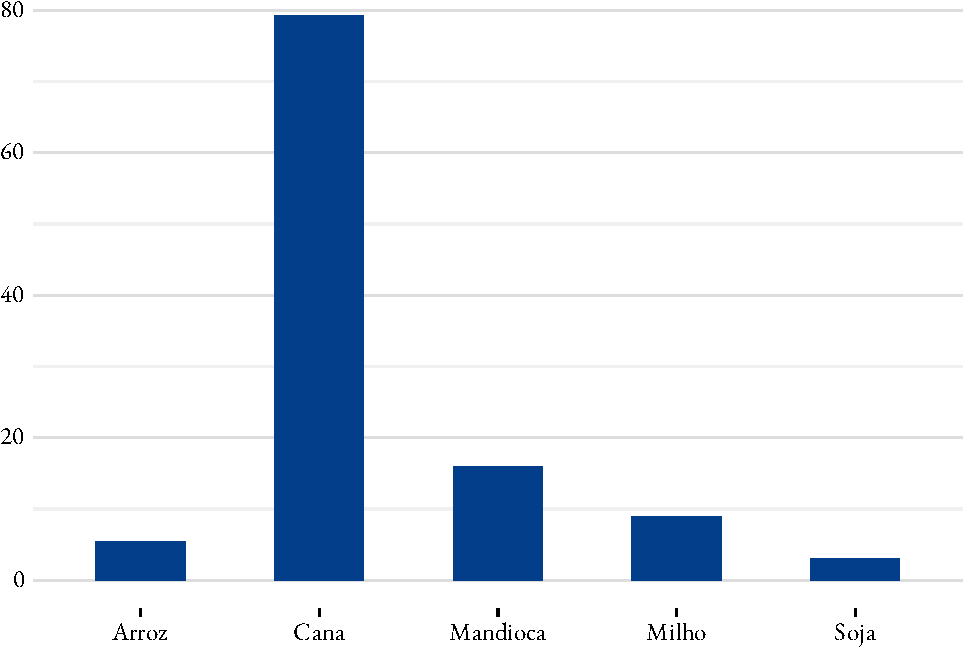
\includegraphics{fig/rendim_medio-1.pdf}
		\source{\acrshort{sidra}/\acrshort{ibge}}
		\label{fig:rendimento}
	\end{subfigure}
	\begin{subfigure}{\linewidth}
		\caption{Área plantada das lavouras}
		\subcap{Em mil hectares. Estimativa anual de setembro}
		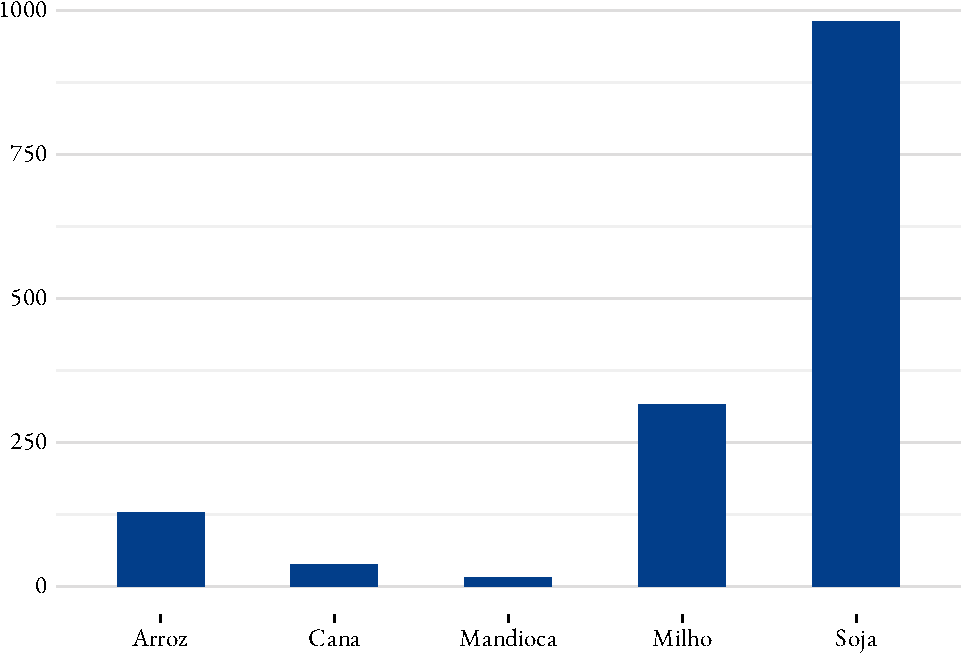
\includegraphics{fig/area_plantada-1.pdf}
		\source{\acrshort{sidra}/\acrshort{ibge}}
		\label{fig:areaplantada}
	\end{subfigure}
\end{figure}

% \section{Rendimento Médio}
\par Dentre os cinco principais produtos cultivados na agricultura tocantinense, o rendimento médio demonstrado na Figura \ref{fig:rendimento} mostra como as características próprias de cada um deles tem resultado determinante no cálculo da área que deve ser plantada, visando a quantidade em que será colhida. O cálculo é feito pela divisão entre quilogramas colhidos pela área plantada, significando que, quanto maior o valor do rendimento médio, menor é a área necessária para sua colheita. Sendo assim, os dados mostram que o maior rendimento médio entre estes produtos é da cana-de-açúcar, chegando ao elevado valor de 70,7\%. O segundo produto é a mandioca, com um rendimento médio de 14,3\%, seguido pelo milho, ao total de 7.7\%, arroz, com 4,7\% e por fim, a soja, com um rendimento médio de 2,6\%, ou seja, precisando então de uma vasta área plantada para colher sua quantidade desejada.

% \section{Áreas plantadas e colhidas}

\par Baseando-se no primeiro semestre tem-se os dados das áreas plantadas e colhidas, apresentado na Figura \ref{fig:areaplantada} e consequentemente, os cereais e oleaginosas que mais usam o espaço tocantinense para a produção. No primeiro semestre de 2020, o Tocantins utilizou-se de 1.427.342 hectares para plantação. O maior espaço disso é para a Soja que utilizou-se de 975.513 hectares para a produção, demonstrando que a soja utiliza-se de uma grande quantidade de hectares para a sua produção. Então, a soja tem 68.7\% de utilização do espaço de plantio, em seguida vem o milho que utiliza 18.8\% do território, os dois espaços mais usado para a plantação. O arroz corresponde 8.8\%, em seguida cana com 2.7\% e mandioca com 1\%.

% \section{Produção de leite}
\par O estado tocantinense é conhecido pela sua produção agropecuária e os seus derivados. A fabricação de leite em solo tocantinense no ano de 2019 foi de 132.237 (mil litros), apesar de uma produção grande, o estado ainda não se tornou referência no segmento ficando com menos de 1 percentual na produção do Brasil. O estado mantém valores constantes na sua produção, e não apresenta grande variação nos últimos cinco trimestres. Por fim, sua produção no primeiro trimestre do ano de 2020 teve uma produção de 37.273 (mil litros), apresentando um aumento pequeno comparado ao valor do quarto semestre de 2019 que teve uma produção de 36.369 (mil litros).
\begin{smbox}[label={labelbox},nameref={Agricultura}]{Produção em evidência e Agronegócio em geral}
	O estado do Tocantins tem uma economia pautada no agronegócio (não apenas a do Tocantins, a brasileira em si). Com as frequentes desvalorizações cambiais recentes, tornou-se atrativo produzir commodities como a Soja. O câmbio e a qualidade do solo justificam o desejo de se produzir soja no Tocantins. O argumento da riqueza gerada pela soja pode ser visto na sessão em que é apresentado os balanços de pagamentos estaduais, e o valor que esse produto gera ao estado.
\\
	No Brasil existem inúmeros órgãos que cuidam e divulgam dados sobre agricultura, sejam municipais, estaduais ou federativo. Uma referencia impar destes dados é o \acrshort{sidra} (Sistema IBGE de Recuperação Automática). Outra referência para agricultura é o \acrshort{ipea} (Instituto de Pesquisa Econômica Aplicada), além das secretarias estaduais e municipais que realizam pesquisas próprias. No Tocantins, a \acrshort{fieto} (Federação das Indústrias do Estado do Tocantins) e a secretaria da fazenda do estado realizam pesquisas similares.
\end{smbox}

\par Já o setor de abate de animais apresenta resultados significativos para a economia estadual. Analisando esse setor, a Figura \ref{fig:abate} apresenta dados a partir do trimestre de 2019. Compreendendo o semestre do ano vigente, é apresentado um bom primeiro trimestre (antes do efeito da pandemia e o isolamento social), na qual, o Tocantins apresentava a sua melhor performance no abate de animais, sendo conduzido pelo abate de aves, em que passou de 4.000 mil cabeças de aves no primeiro trimestre. Bois, novilhas e vacas tiveram resultados constantes. Já no segundo trimestre, os resultados foram ruins e desconexos com a série histórica, porém, a justificativa desse resultado ruim é o efeito da pandemia na economia. O que demonstra que nesse primeiro semestre, o trimestre inicial apresentou ótimos resultados e o segundo foi ruim.


\begin{figure}[!h]
	\caption{Abate dos principais animais}
	\subcap{Mil cabeças}
	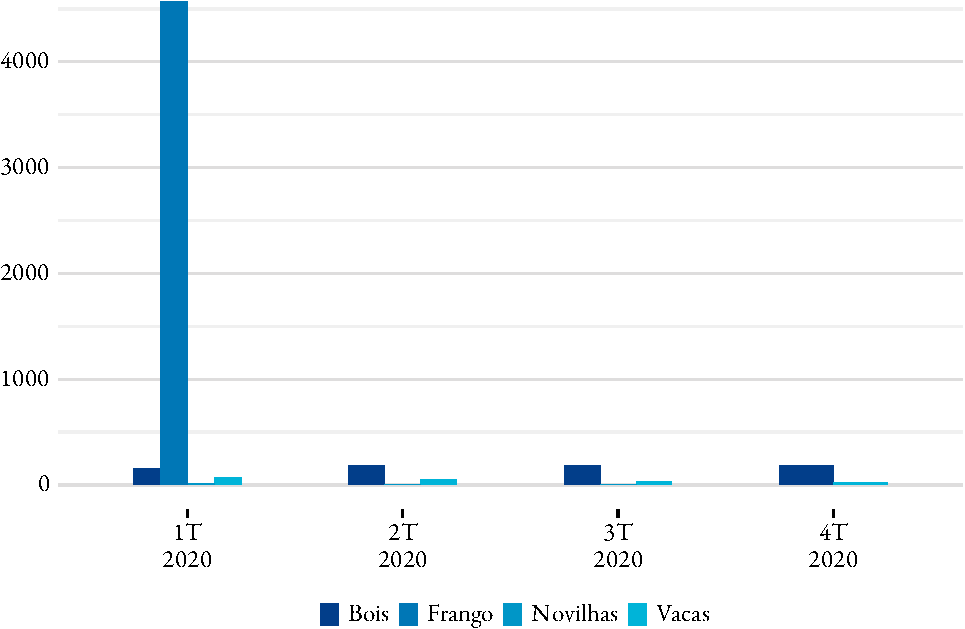
\includegraphics{fig/abates-1.pdf}
	\source{\acrshort{sidra}/\acrshort{ibge}}
	\label{fig:abate}
	\notes{\trimestres}
\end{figure}
